\documentclass[a4paper]{article}

\usepackage[T1]{fontenc}
\usepackage[utf8]{inputenc}
\usepackage{courier}
\usepackage{graphicx}
\usepackage[justification=centering]{caption}
\usepackage{listings}
\usepackage{color}
\usepackage{pdfpages}
\usepackage{algpseudocode}
\usepackage{algorithm}
\usepackage[colorlinks=true,linkcolor=blue,citecolor=blue,urlcolor=blue]{hyperref}
\definecolor{mygray}{rgb}{0.5,0.5,0.5}

\title{Online reputation management}
\date{\today}
\author{Cecilia Roes \\ Simon Österman \\ Alexander Gomez \\ Tang-Chu Chen \\ Viktor Gavelli}

\begin{document}
\maketitle
\begin{abstract}
This paper describes an implementation that harvests data from twitter for sentiment analysis regarding a certain organization or product. 

- What is described and implemented 

For harvesting tweets we used the Twitter API....

Classifier - Naive Bayes

Before training the classifier with the twitter data, the data was pre-processed to more effectively and accurately get processed. 

- Conclusions/Results

\end{abstract}
\newpage
\tableofcontents
\section*{Contributions}
Alex and Viktor have been responsible for the tweet harvesting.
Simon the preprocessing, Tony the feature extraction and Cecilia the classifier and producing the results.

Everyone has contributed to the report in their area, but also helped out on areas not covered by anyone.
\newpage
\section{Introduction}
A company’s reputation has always been an important asset. Today there are new opportunities to follow changes in reputation as a reaction to specific events by monitoring social media. However social media produces huge amounts of data, too much to be processed manually, so there’s a need to find other ways of automatically processing it.

The problem this report explores is; How can we detect (event or product) impact on a company’s reputation using twitter?

How does one determine how a tweet affects reputation? If the sentiment of the tweet is positive we are going to assume that it’s going to have a positive impact on reputation, and the opposite effect for tweets with negative sentiment. After determining if a tweet has a positive or negative impact we also need to weigh how big of an impact a specific tweet has. The more people read a tweet, the more likely it is to cause a change in peoples perception. If a tweet has been retweeted it usually suggests people agreeing with the sentiment, which strongly indicates the sentiment being important for peoples view of the company.

Using these assumptions we can attempt to solve the problem by sentiment analysing tweets, giving them weight according to importance and then aggregating the resulting reputation impact by company. If this is done over time, one can monitor reputation changes as a result of events and happenings, such as product launches or movie premieres.

\section{Related work}
There are several existing tools for Online Reputation Management, such as SAS Sentiment Analysis \cite{SAS}, SocialView \cite{SocialView} and even simpler free ones like SMM \cite{SMM}. Some are open source and have detailed descriptions of the algorithms used, while others not. A common factor is that they all in some way use sentiment analysis to process social media content.

Sentiment analysis uses linguistics, natural language processing and text analytics to extract opinions from a text. This is a growing field and there are still a lot of problems to solve, making a computer understand human language is very difficult, and it is outside the scope of this report to discuss these problems in detail. If interested some of the issues and considerations are discussed by Pang and Lee in their book Opinion mining and sentiment analysis \cite{PangLee}. They discuss sentiment polarity and the fact that a text could be classified as other things than positive or negative, f.eg. angry or sad. It also discusses the problem with subjectivity and objectivity, the importance of determining features of a text and the problem of negation.

\subsection{Sentiment analysis algorithms}
All popular algorithms for sentiment analysis are machine learning algorithms. The most commonly used ones are Naive Bayes classifier, Maximum Entropy classifier and Support Vector Machines. As more labelled data has become available, extensive evaluations have been done of these, f.eg.  by Pang et al.\cite{Pangetal} for movie reviews.

One important thing to be aware of when looking at sentiment analysis algorithm performance is that humans only agree about 79\% of the time \cite{79percent}.

\subsubsection{Naive Bayes classifier}
Naive Bayes is a probabilistic classifier based on Bayes’ theorem. The naive part is that it assumes that each features existence is independent on any other feature, this may not always be true. One big advantage with the Naive Bayes is that it does not require very much data for training. Since the features are considered to be independent of each other, there is only the variances of each feature belonging to the class (positive/negative) which needs to be trained to obtain the trained classifier \cite{bayes}.

\subsubsection{Maximum Entropy classifier}
Maximum Entropy is another probabilistic model which could be used as a classifier. Unlike the Naive Bayes classifier, it does not assume statistical independence of the features. This difference theoretically makes the Maximum Entropy Classifier more accurate but at the price of speed. Without the assumptions, the classifier takes more time and requires more data to train and may therefore not  be suitable for big volumes of classes. For further reading and the mathematical model see \cite{max_ent}.

\subsubsection{Support Vector Machines}
Support Vector Machines is a non-probabilistic model for classification \cite{svm}, unlike the two models described previously. The training is done by feeding input marked with one out of two classes. A training algorithm assigns the input to the indicated class and builds a model based on this data. The model is represented as points in space. The points of the two classes should be divided by an as large “gap” as possible. New input is then placed in a class depending on which side of the gap it lands.

\subsection{Twitter}
Most of the previous sentiment analysis’ has been done on longer texts, such as restaurant or movie reviews. Trying to analyse tweets is very different and in some ways more difficult. There are fewer and less extensive training sets available for this use case and the short length of the tweets also makes training more difficult. The language of tweets is also often full of abbreviations, incorrect language and duplicate characters such as in ‘sweeeet’, causing trouble for the analyser. Go, Bhayani and Huang discuss this in an article \cite{twitter_ds} detailing sentiment analysis of tweets using distant supervision. They take advantage of these special characteristics of tweets and use tweets containing emoticons as training data. By assuming happy emoticons (‘:)’, ‘:-D’) indicate positive sentiment and negative emoticons (‘:(‘) the opposite you can easily gather a large training set without any manual labelling.

\subsection{Weighing of Tweets}
When dealing with tweets, one question appears: should we weight all our tweets the same? In our life experience, the opinion of an expert weight more than a nobody’s opinion. Therefore, weighting tweets with different value is a intuitive idea. Pagerank is a good algorithm for finding relevant and important web pages, so trying to develop a weighting algorithm from pagerank seems to be a good idea.

The main idea of pagerank algorithm is that the probability a user jump from node i to node j is influenced by two main factors. First, the links in node i and econd, a random jump from node i to node j.

Therefore, it seems reasonable to use a similar idea when trying to weight tweets and we found a report \cite{weight2} detailing such an approach.

A user “jumping” from a tweet to another is influenced by many functions that twitters provided, for example, the function of retweet, of mention, of hashtag and of follower.

Therefore, we can rewrite our “probability matrix” in;

\[G = aR + bL + cM + dF + eH\]
\[(a + b + c + d + e = 1)\]
where R represent the probability matrix of random walk, L(i,j) represent a user accessing tweet j by following a retweet on tweet i, M(i,j) represent a user accessing tweet j by following a mention on tweet i, F(i,j) represent a user accessing  tweet j because the writer of tweet j is a follower of tweet i, and H(i, j) represent a user accessing tweet j because both of the hashtag s of tweet i and tweet are the same.

It seems to be a reasonable way to model the behaviour of twitter users.

\section{Method}
\subsection{Tweet harvesting}
We chose to harvest the tweets using the newer v1.1 Twitter API \cite{tw_api}. Whilst the newer API requires authentication, it does allow for a much greater harvest rate. The older v.1 Twitter API \cite{tw_api_1_0} only allowed 150 requests per hour unauthenticated and 350 per hour if authenticated. The newer API allows 450 requests per 15 minutes if you authenticate yourself. With GET search able to return a maximum of 100 tweets per request, we are able to harvest 45,000 tweets every 15 minutes. This allows us to get enough data to get a satisfying result within a reasonable time frame.

To be able to notice the change in sentiment over time, we need to constantly harvest tweets. We chose to harvest as many tweets as possible (up to a maximum of 45,000) each day for a week for our chosen brands. We use the same number of tweets (1000) each day for each brand to calculate our results.

\subsubsection{Queries}
The request was configured with ‘count=100’ in order to get the maximum amount of tweets per request. Setting ‘result\_type=recent’ makes sure the result is returned chronologically and ‘lang=en’ lets you get tweets written in english.

Twitter's search function have a built in filter for positive and negative emoticon search. This simplifies the process of searching for all permutations of the positive or negative smiley. Using the search query “:)” for the positive and “:(“ for the negative returns the wanted tweets for our training data. It’s possible to remove retweets with a “-RT” in the query, this doesn’t work all the time and therefore it also had to be looked for in the preprocess stage. 

For the brands, we used the GET Search function from the twitter api and simply searched for the brand we were interested in. We included common variations, for example in the case of Iron Man we searched for ‘“iron man” OR iron\_man OR ironman’ in order to get a more complete result.

\subsubsection{Storing tweets}
The obtaining of tweets has to be done in several steps. To simplify the whole process we chose to save these tweets in a database. This simplifies the storage of tweets and later filtering depending of what will be used. Such values as number of retweets and number of favourites is stored and can be extracted from the database. Having the tweet id in the database helps prevent duplicates of the same tweet. It can also be used to continue a previous search by using it in the query by using “since\_id” or “max\_id”. The database also saves the time at which the tweet was made and is later used to group the tweets for each day.

\subsubsection{Restrictions of the Twitter API}
Twitter have only 6-9 days of Tweets available for search request. This search function have flaws as stated by Twitter: “The Search API is not complete index of all Tweets” \cite{tw_search}, therefore the search process has some inaccuracy. Depending on the search query there are different amount of tweets made every day which makes it difficult to obtain a constant amount of tweets per day.

\subsubsection{The authentication process}
The Twitter API uses Oauth for its authentication, we chose the application only authentication because of its high limit. To utilize this authentication, an account for the program needs to be registered with Twitter, this grants us access to a consumer key and and a consumer secret that we use in our bearer token extraction. The bearer token is then attached to each HTTP Get request that is made for our query. Twitter responds to our Get request with tweets in a Json structure with a maximum of 100 tweets per response. Our bearer token is valid until it is invalidated by us.

\subsection{Sentiment analysis}
We chose to implement the sentiment analysis using Python and the nltk library \cite{nltk} using the built-in NaiveBayes classifier. For simplicity we decided to interpret all opinions as either positive or negative, while in reality things aren’t usually that black or white and having a multistep scale would better reflect real sentiment.

\begin{algorithm}
  \caption{Sentiment analysis algorithm}
  \begin{algorithmic}
    \Procedure{createClassifier}{positiveTweets, negativeTweets}
      \State trainingSet, testSet = preprocess(positiveTweets+negativeTweets)
      \State extractFeatures(trainingSet)
      \State classifier = trainClassifier(trainingSet)
      \State print classifier.accuracy(testSet)
    \EndProcedure

    \Procedure{analyse}{company, date, tweets}
      \State \textbf{return} [company, date, classifier.analyse(tweets)]
    \EndProcedure

    \Procedure{main}{}
      \State createClassifier()
      \State results = [] 
      \For {$f$ in $files$}
        \State result.append(analyse(f.company, f.date, f.tweets))
      \EndFor
      \State display(results)
    \EndProcedure
  \end{algorithmic}
\end{algorithm}

The preprocessing and feature extraction is discussed in further detail below. As stated earlier we used nltk for the classifier \cite{nltk_book}, we train it and run an accuracy test on a set obtained in the same way as the training set, then we analyse files with tweets about certain companies.

The results from the analysis we display using a simple python web server and Google charts. The entire sentiment analysis implementation including instructions of how to run it can be found on github \cite{github}
\\
\\
Originally we wanted to assign a weight to each tweet depending on its influence but unfortunately we didn’t have time to implement that.

\subsubsection{Training set and preprocessing}
As mentioned above, the tweets require some preprocessing in order to be effective input to the classifier. 
Which processing that is done depends on the type of data that is being processed. In the case of training data:

 The formatting of the training data is done in two steps:
1. Removal of unwanted tweets.
2. Editing of certain words.

The tweets that we do not want to use as training data are retweets and tweets containing both positive and negative emoticons. A retweet is considered to be any tweet containing the word “RT” which is usually used in tweets to highlight that something is being retweeted. Those tweets should not be considered in our training data to avoid certain tweets gaining extra weight.
Tweets containing both “happy” and “sad” emoticons can not automatically be determined to be of either positive or negative sentiment. Therefore, we do not want to use these tweets to train our classifier.  

Removing these tweets are only done for our training data. The editing of words however are done for both training data as well as for analysing data. The editing is done on some features which are common in tweets. Such features are usernames (indicated by an @-prefix) and links. Since we are training our classifier with tweets containing emoticons, we want to remove these before analysing to avoid them getting too high weight in our classifier. 
Words with more than two of the same letter in a row are being cut down to two of that letter to avoid getting many different representations for the same word which saves time for the analysis.

\subsubsection{Feature extraction}
Considering all words in training data as features is not an efficient method. Many of the words in users’ comment have little correlation with positive or negative. Therefore we can use feature extraction to speed up the implementation \cite{elim_features}.

The method we used for feature extraction is combined with the Pearson's chi-square test from Statistical hypothesis testing \cite{chi-square}. For a word in the training data, we want to find out whether it has a strong correlation with positive or negative. If a word occurs only in our positive training data, then we have a very good reason to believe that the word is a good feature. On the other hand, if we encounter a word that occurs both in the negative and the positive data set with equal frequencies, then we might doubt that it is a good feature.

So for every different word, we try to calculate the chi-square value with the null hypothesis as “the word has no correlation with positive nor negative”. The higher the value is, the more confident we can be in that it will be a good feature. Therefore we sort our words by the chi-square value and select those word with larger value.

Chap 5.3.3 of the book “Foundations of Statistical Natural Language Processing“ \cite{foundations} suggests we should use chi square test instead of t test. Because the probability distribution of a word’s frequencies is not believed as a normal distribution, chi square test is more appropriate in our case.

\begin{algorithmic}
\For {a word w}
  \State H0 : occurrence of w is independent to positive opinions( and negative opinions )

  \Comment{We calculate the marginal probabilities,}

  \State Let N = numbers of words in our all data

  \State P1 =  frequency of w in all data / N
  \State P2 =  frequency that words in our all data is not w / N
  \State P3 =  frequency that words in positive data / N
  \State P4 =  frequency that words is not in positive data / N

  \Comment{with those marginal probabilities, we can calculate our “expect values” under the assumption that occurrence of w is independent to positive opinions ( and negative opinions).}

  \State Let s be a random variable representing a word is w,
  \State t be a random variable representing a word is in positive opinion:
  
  \State E( s \& t ) = P1 * P3
  \State E( s \& ~t ) = P1 * P4
  \State E( ~s \& t ) = P2 * P3
  \State E( ~s \& ~t ) = P2 * P4

  \Comment{Along with our “observe value” which are:}

  \State O( s \& t ) = frequency that the word w in positive data / N
  \State O( s \& ~t ) = frequency that word w in negative data / N
  \State O( ~s \& t ) = frequency that a word except w in positive data / N
  \State O( ~s \& ~t ) = frequency that a word expect w in negative data / N

  \Comment{By calculating the following equation, we’ll get the chi square value of the word w. The higher the value is, the more confident we believe that word w has a certain correlation with positive sentiment.}

  \State Chi-square value = 
  \State [ O( s \& t ) - E( s \& t ) ]\^2 / E( s \& t ) +
  \State [ O( s \& ~t ) - E( s \& ~t ) ]\^2 / E( s \& ~t ) +
  \State [ O( ~s \& t ) - E( ~s \& t ) ]\^2 / E( ~s \& t ) +
  \State [ O( ~s \& ~t ) - E( ~s \& ~t ) ]\^2 / E( ~s \& ~t ) 
\EndFor
\end{algorithmic}

\section{Results}
\subsection{Accuracy}
Our implementation included measuring the accuracy of our classifier, this is done using a test set retrieved in the same manner as the training set. We have seen that the accuracy improves if the number of features increases, this is likely to be true up to a certain limit as our implementation uses the top most informative features, if too many features are used we’re also going to use low information ones. Currently we’re using about 30000 tweets to train the classifier, this is not a lot for a distant supervision method, using more training data would likely also improve the accuracy. Because of limited time and computer resources we haven’t been able to experiment with this, but with our current setup we reached an accuracy of 77.35\% which compared to the approximated human agreement of 79\% isn’t bad.

\subsection{Reputation management}
The charts are a product of eight days of tweets about four currently relevant brands that were analyzed. 

As can be seen Iron Man surprisingly got very negative results, even though in our opinion while reading a subset of the tweet they seemed generally positive or neutral. The other brands get both positive and negative values though, which leads us to believe there isn’t anything inherently wrong in our implementation, but factors such as weighing everything as positive or negative (not neutral) and a limited training set might be the cause. We also tried running the Iron Man data using a training set where the emoticons weren’t stripped, this gave positive results for Iron Man as well.

The daily reputation value shows the reputation for each date which is good for tracking immediate event response. Although a reputation for a day may have many reasons, big events such as premieres and product releases do have a strong correlation to reputation. Reputation can be seen as a single value that changes over time, then a daily reputation value chart with a short timespan as a week doesn’t say anything about the real reputation value of a brand. The accumulative reputation value shows the reputation value over time which changes depending on the reputation each day. Displaying the results in this fashion raises questions about where to start each brand and how to realistically reflect reputation change for each day. Devalue old tweets in the accumulation of the current brand reputation value will hinder such values that won’t change significantly for events with big impact.

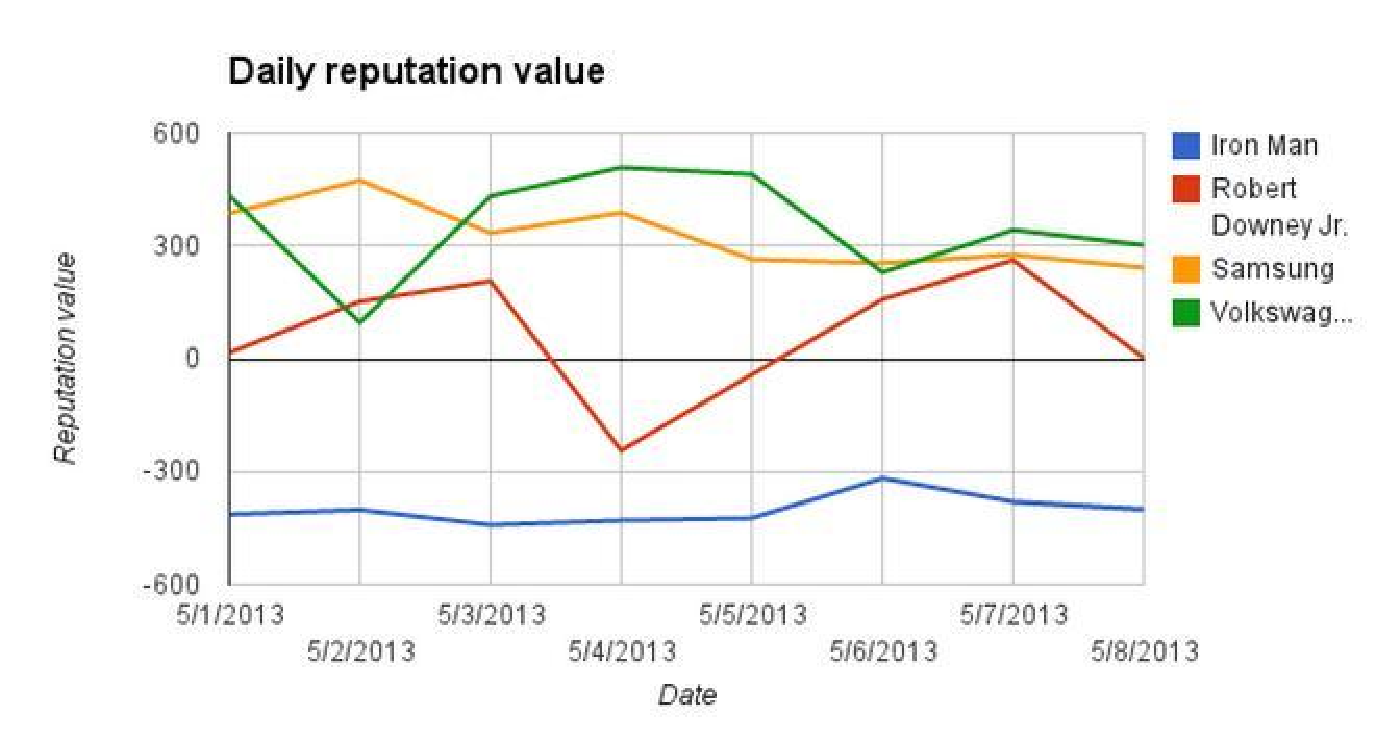
\includegraphics[scale=0.6]{graph1.pdf}
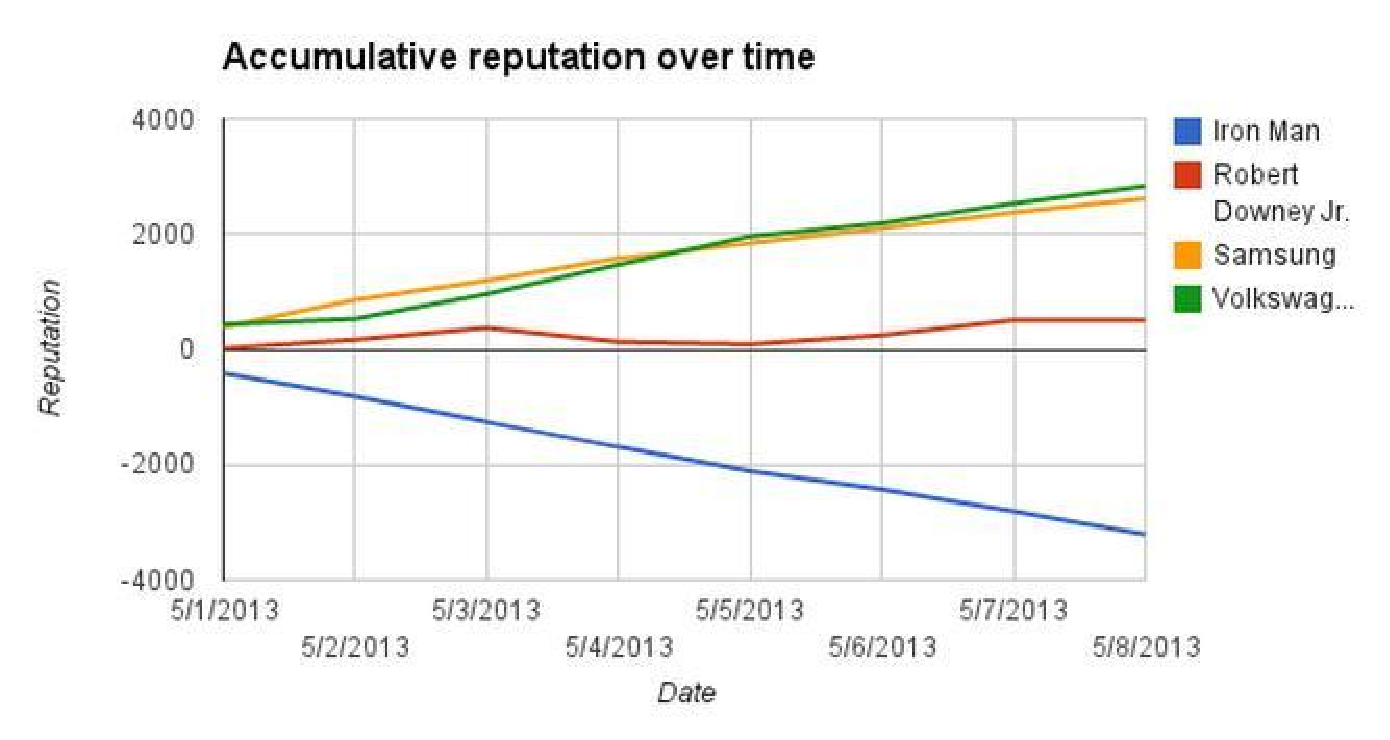
\includegraphics[scale=0.6]{graph2.pdf}
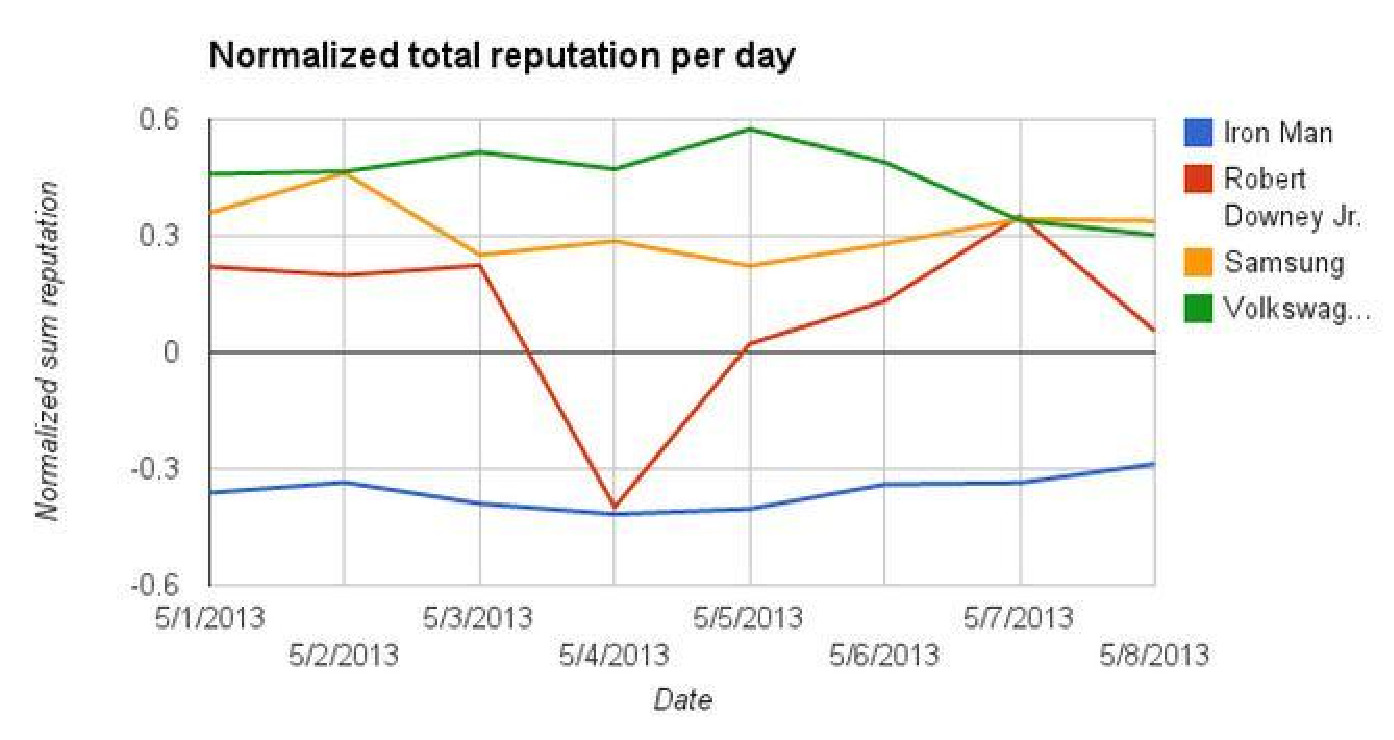
\includegraphics[scale=0.6]{graph3.pdf}

\section{Discussion}
Our analyser produced good results for the test set, and they were improved by increasing the amount of features used and the size of the training set. Given how machine learning algorithms work this is as expected. Selecting relevant features for the classifier is very important, and since the training data was labeled as positive or negative on the basis of it containing certain emoticons we decided to strip the emoticons from the training set to not cause them to have too high of an impact, making all other words irrelevant. This might’ve caused some adverse effects, emoticons are still good indicators of sentiment, and a better approach would probably have been to keep the emoticons in a subset of the training set. This at least partly explain the Iron Man results and suggests a way to likely make them more reasonable.

Our sentiment analysis evaluates tweets as either positive or negative, there is no in between. At least being able to also assign tweets as neutral would make the analysis more realistic. The problem is how to produce the extra training and test data needed, preferably without having to label tweets by hand.

Another way to improve the result could be to assign weights to individual tweets. Our idea was to assign higher weights to frequently retweeted tweets and tweets written by more popular tweeters. This would improve the result by reflect how influential a tweet is to a company's reputation. It could also be discussed if positive and negative tweets should have the same weight, as the saying goes ‘no publicity is bad publicity’.

\bibliographystyle{plain}
\bibliography{refs}
\end{document}

